\chapter{Methodology}

In this chapter the methodology including the used concepts such as survey for user segmentation, paper prototyping for usability testing and elicitation of requirements is described. Finally, we describe the design methods for the catalogue of design principles.

\section{Survey for User Segmentation}

The questionnaire that we created for finding test users for the Paper Prototyping Session follows the design guidelines of Andrews et al. \cite{andrews2007conducting}. The guidelines say that electronic surveys should be designed to...

\begin{itemize}
	\item support multiple browsers and platforms \cite{yun2000comparative}
	\item prevent submitting multiple times \cite{yun2000comparative}
	\item to present questions in an adaptive or logical manner \cite{kehoe1997eighth}
	\item allow saving the work in long questionnaires with more than 50 questions \cite{smith1997casting}
	\item collect both quantified selection option answers and narrative type question answers \cite{yun2000comparative}
	\item have the possibility to thank the users for completing the survey \cite{smith1997casting}.
\end{itemize}

Google Form is a web application out of the Google Web Apps that follows all these guidelines, which was the reason for choosing it for our survey.

As the motivation to find subjects who completes a survey increases as the question difficulty increases \cite{andrews2007conducting}, when the aim is to have numerous replied questionnaires the survey should comprise of simple and not to much questions.

Generally online survey platforms offer convenient and reliable data management \cite{carbonaro2000design}. By design, Google Form protects against the loss of data and facilitates data transfer into a database, in this case Google Spreadsheets for analysis.

Before sending out the survey and after deciding on the survey tools, contents and platforms it is very important to carry out a pilot \cite{lumsden2007online}.

\subsection{Evaluation of the Questionnaires}

The user segments on which this thesis builds upon are described in \ref{chap:usersegmentation}. Smart Cities Demo Aspern did a survey and used cluster analysis to define clusters. These clusters had distinct features. The answer of one user of the questionnaire can then be evaluated against each user segment with it's distinct features. This evaluation amounts to a correspondence of one answer set to a user segment.

According to Kazi and Khalid \cite{kazi2012questionnaire} there are three types of validity, which is the degree to which an assessment measures what it is supposed to measure. The three types are content validity, criterion-related validity and construct validity. The validation technique for identifying the correspondence of a user to a user segment is the criterion-related validity as it best describes the equivalence to the segment characteristics.

\section{Elicitation of Requirements with Paper Prototyping}
  For the Paper Prototype a Step-by-Step guide proposed by Arnowitz et al. \cite{arnowitz2010effective} is used. To create a Paper Prototype the following steps should be done:

\begin{enumerate}
	\item \textbf{Create scenario}. Before starting to draw anything the main user goals and tasks have to be portrayed. This can be done in a scenario narration.
	
	\item \textbf{Inventory UI elements}. The next step is to make a checklist of all UI elements that may be needed to support the scenario
	.
	\item \textbf{Create UI elements}. All the UI elements from the checklist from the previous step are now created in paper form. There are a lot of tools and materials that can come in handy at this step. The following list of materials might help the process: paper, sticky notes, whiteboard, sketchbook, notebook, napkin, cards, overhead sheet, cardboard, carton, scissors, markers, UI stencil, correction fluid and tape and transparency sheet. 
	
	\item \textbf{Run through scenario}. In this step a dry-run through the scenario with the paper prototype should be done and missing parts should be found an recreated.
	
	\item \textbf{Internal review}. The last step in the first round is the internal review with the team where the audience is defined, the goals for each version of the prototype is reviewed, the expectation of the reviewers are found out and the next steps are planned.
\end{enumerate}

The next Step-By-Step Guide is following the first. It was also proposed by Arnowitz et al. \cite{arnowitz2010effective} and is for testing the Paper Prototype:

\begin{enumerate}
	\item \textbf{Revise scenario}. The internal review may have uncovered some tweaks that you want to change. Be careful for changes at the scenario as it may cause a ripple effect which can lead to necessary changes in user interface elements or even new screens. Keeping changes to minimum is recommended. If changes are necessary keep in mind that this can lead to non comparable results in the end.
	
	
	\item \textbf{Revise inventory UI elements}.
	Until now maybe multiple run throughs through the prototype have been done and you noticed that some vital pieces of the interface are missing. Now is a good time to check completeness of the UI elements checklist. Developing a set of UI elements for cases that you did not anticipate may be also useful.
	
	\item \textbf{Create UI elements}.
	Check if the collection of the UI elements is still complete and create some more if needed.
	
	\item \textbf{Pilot run through scenario}. Before presenting the prototype to the user it has to be tried out first. You can give the Prototype to anyone, e.g. a team member, to try it out. The aim here is to find missing pieces to be prepared for everything they do. The run through will ensure that you haven't created a half-baked prototype.
	
	\item \textbf{Internal review}. 	
	In this step the scenario and the prototype supplies are revised again with the team. Also the goals and the expectation of the reviewers are revised.
	
	\item \textbf{Prepare Kit}. Before running the prototype session the papers have to be arranged in a way that makes it easy to find the various UI elements. Also blank paper, sticky notes and pens should be prepared for further ideas.
	
	\item \textbf{The Prototype Session}. The user study session is an interactive process where one ore more participants and a facilitator are involved. In a dialogue the participant completes tasks provided by the facilitator. The session is used to get user opinions about early design and task flow ideas represented on paper. The sessions are typically recorded for later examination. The feedback from the users show what they expect from the app which is of great value for the implementation later on \cite{snyder2003paper}. Weiss  \cite[p.~144]{weiss2003handheld} proposes to invite not only one, but two respondents at a time for paper prototype usability tests. He mentions that two respondents feel more comfortable in the casual environment that paper prototyping creates, whereas one single respondent can easily become overwhelmed by the experience.
	
	\item \textbf{Reiterate}. After each prototype session an review and evaluation about what went good and what bad can be done. Although it might be tempting to change things after each session, it is better to wait until all the planned user sessions are done to do an overall comparative review at the end.
\end{enumerate}

\section{Creating a catalogue of design guidelines}

A common challenge is to interpret the results of empirical studies and derive design guidelines which are not too specific but also not too general to make them applicable without additional interpretation effort. The methodology for the deduction of design guidelines for this thesis is inspired by De Bruijn's and Spence's framework for theory-based interaction design. 

\begin{figure}[h]
	\centering
	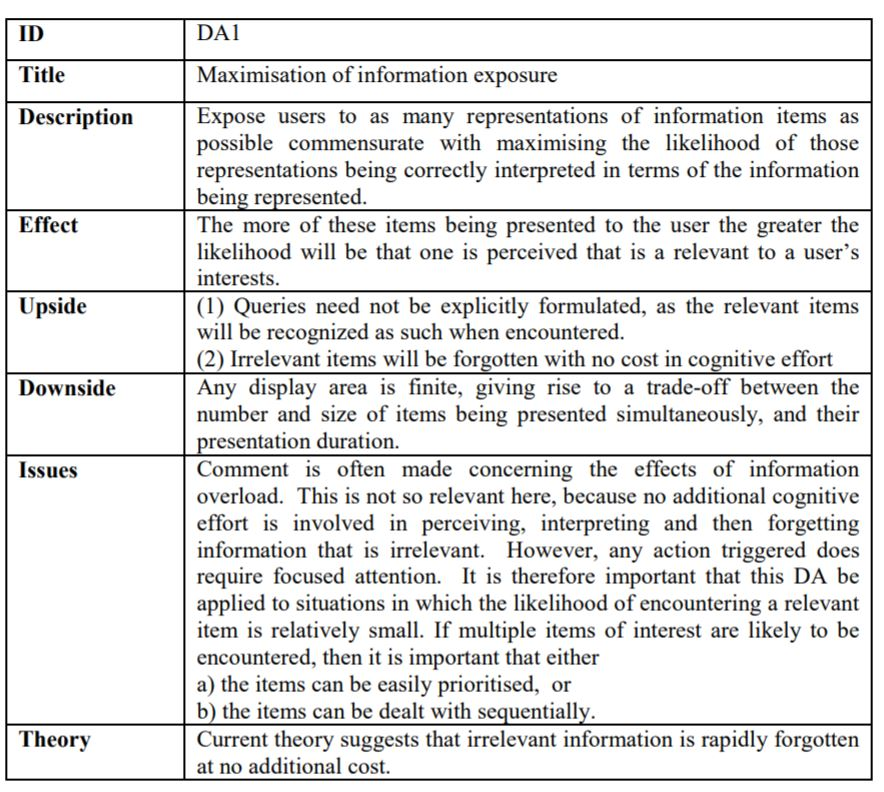
\includegraphics[width=\textwidth]{design_action}
	\caption{Exemplary design action of De Bruijn and Spence \cite{de2008new}}
	\label{fig:designaction} % \label has to be placed AFTER \caption (or \subcaption) to produce correct cross-references.
\end{figure}

The design action is headed by an \textbf{identifier} and a \textbf{title} indicating as clearly as possible the expected result of applying the design action. The \textbf{description} clarifies the brief title, followed by the \textbf{effect} that the design action will have. The design action further includes an \textbf{upside} and \textbf{downside} section that describes advantage and trade-offs respectively. The \textbf{Issues} sections considers issues that are neither positive nor negative. In the last part of the design action the \textbf{Theory} is provided as an opportunity for the designer to dive deeper. Nevertheless, the designer does not necessarily need to understand it in order to apply the guideline.

